\section{Part (b)}
Repeat part (a) for the variable pair provided in "p2b.csv" and compute Pearson correlation $r_b$ and p-value $p_b$. Compare the Pearson correlations $r_a$ and $r_b$ as well as the p-values $p_a$ and $p_b$. Explain your findings: Which variable pair (in part $a$ or $b$) has a stronger association according to the comparison of the correlations? Which variable pair has a stronger association according to the comparison of the p-values? Do the comparisons according to correlation coefficients and p-values agree on which variable pair indicate the same stronger association? If not, why is there such a discrepancy? Next, draw scatter plots (variable 1 vs. variable 2) to visualize  the data for both part (a) and part (b). Which variable pair (in part $a$ or $b$) has a stronger association do you think according to the scatter plots? Does your conclusion agree with the comparisons of the p-values and correlation coefficients? If not, explain why.\\
-----\\

Below is the tabulation of the Pearson correlations and p values as well as scatter plots for each dataset:

\begin{center}
\begin{tabular}{|c|c|c|}
\hline
\textbf{Dataset} & \textbf{Pearson r} & \textbf{P-value} \\
\hline
p2a & 0.3809 & $ 1.04 \times 10^{-83} $ \\
\hline
p2b & 0.9312 & $ 3.74 \times 10^{-49} $ \\
\hline
\end{tabular}
\end{center}

\begin{center}
\textbf{Figure 3:} Comparison of Pearson correlation results between p2a and p2b.
\end{center}

\begin{center}
    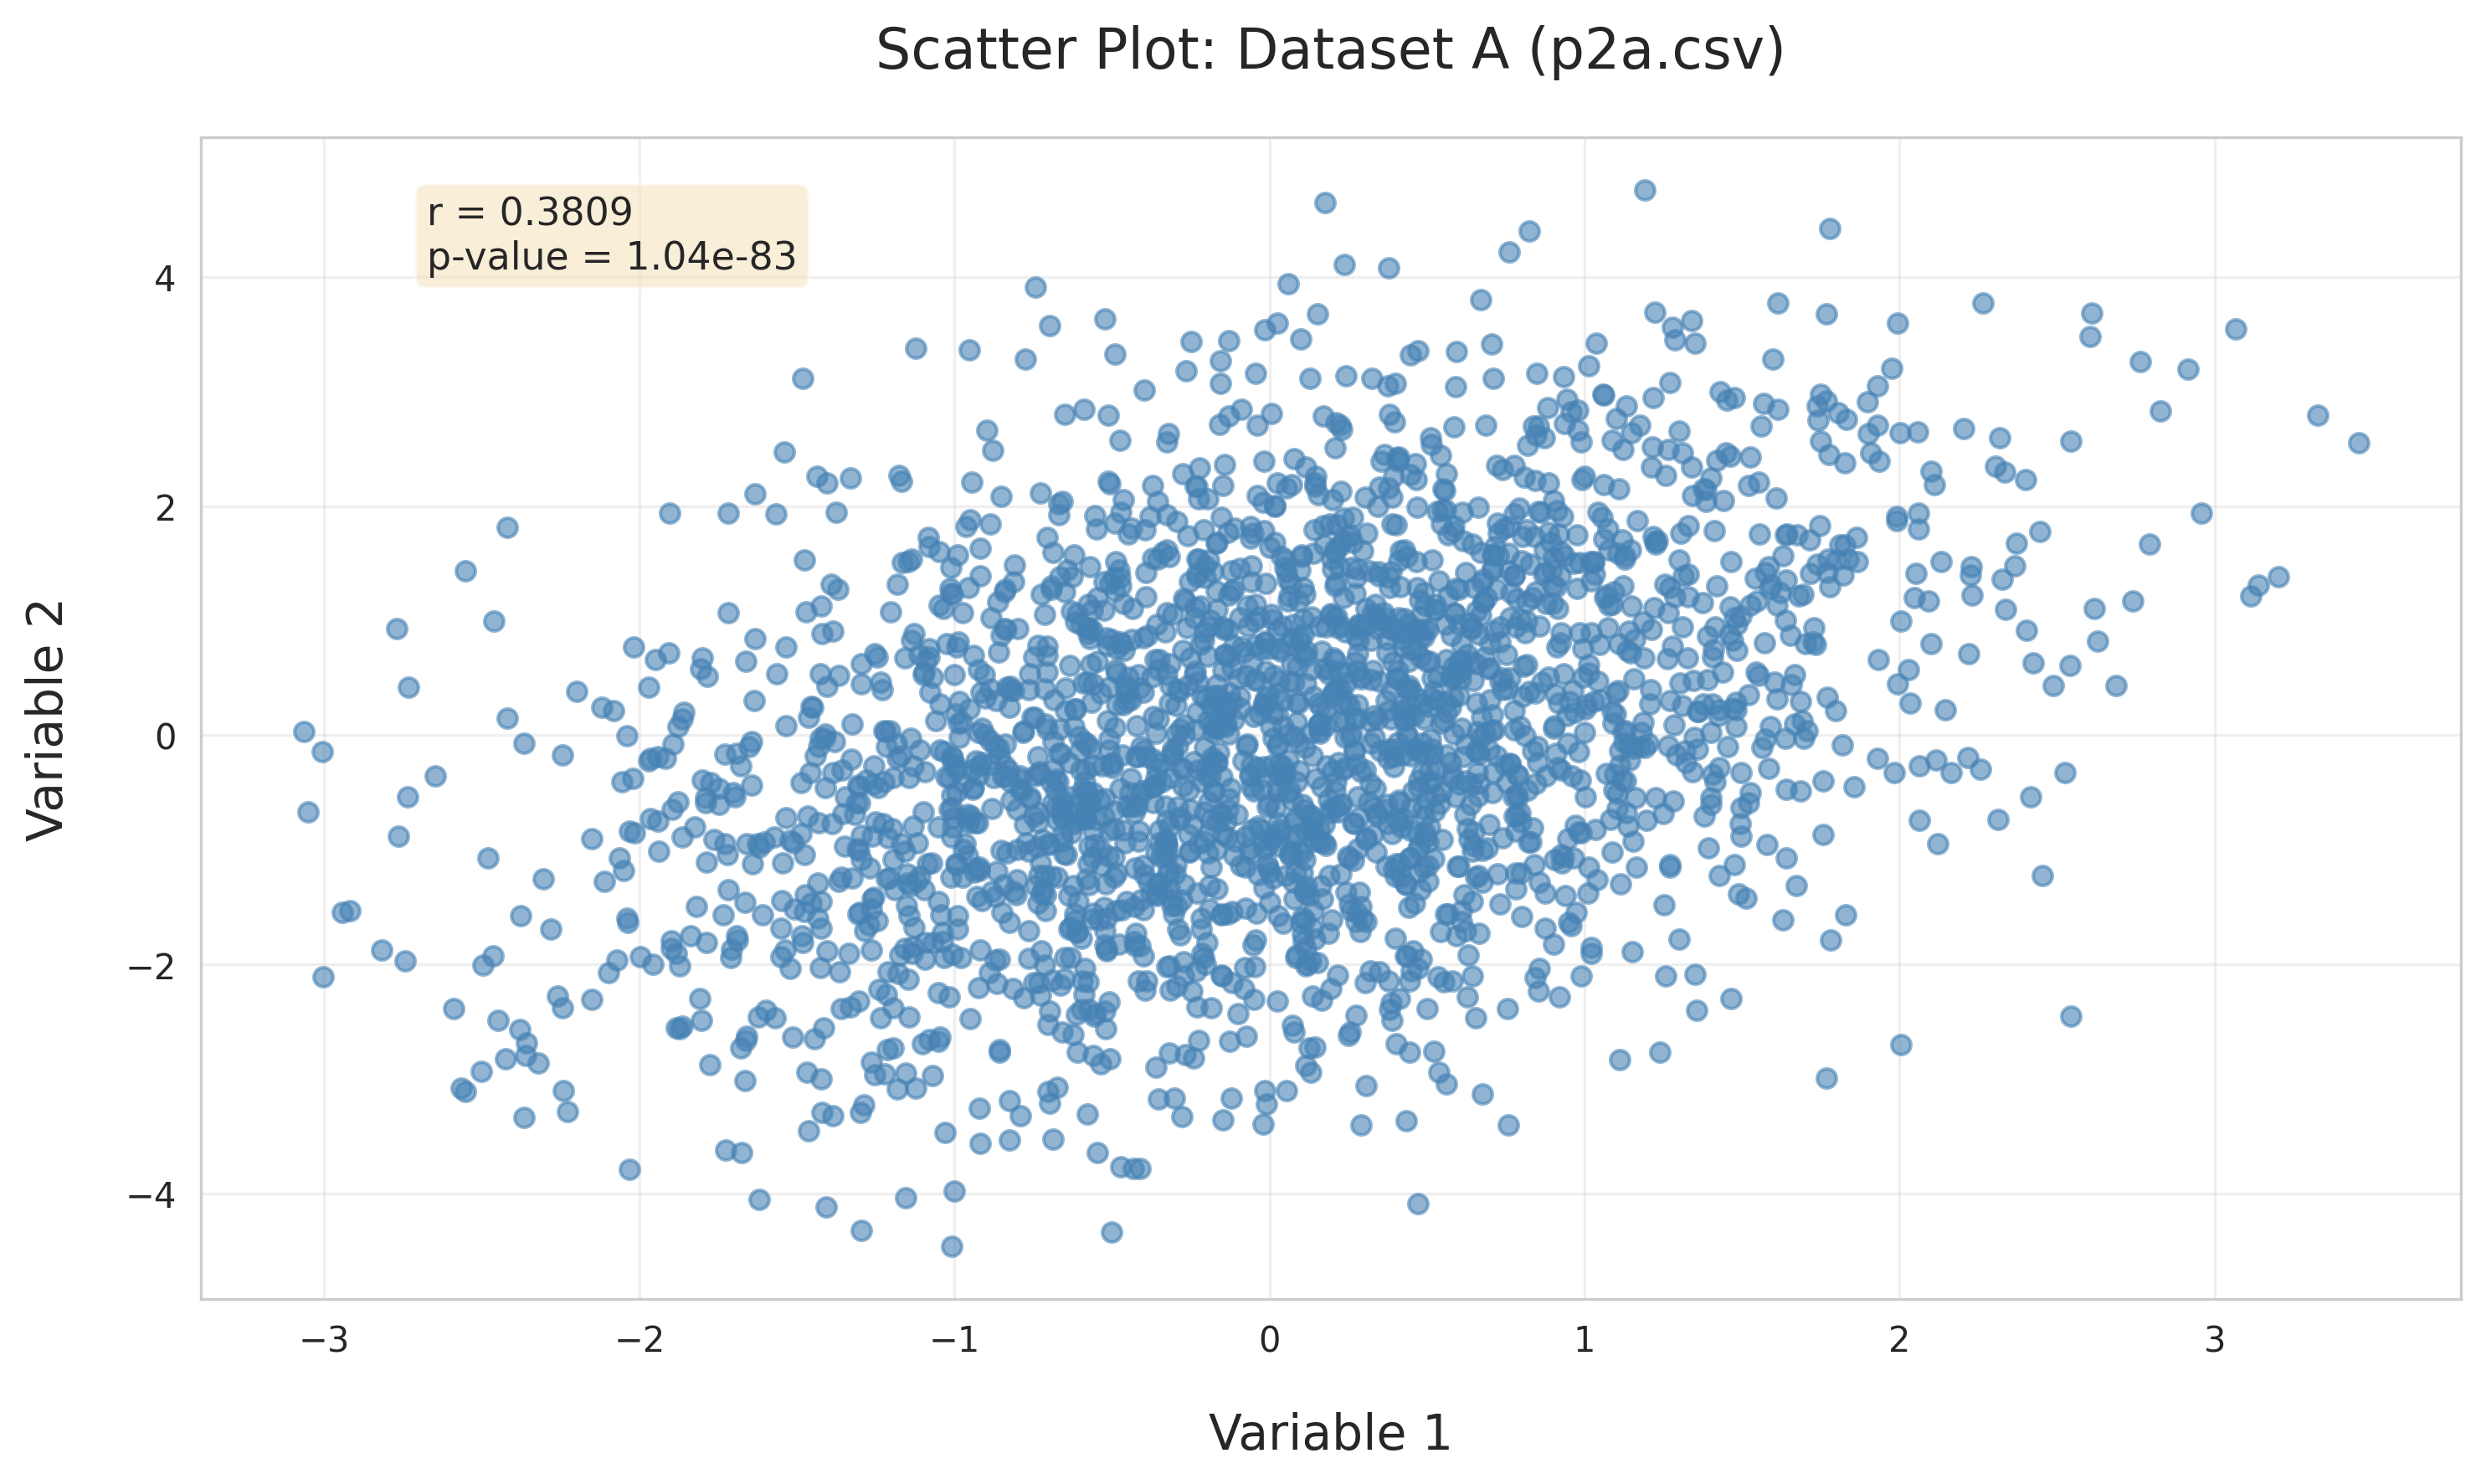
\includegraphics[width=0.95\textwidth]{figures/scatter_p2a.png}
  
    \textbf{Figure 4:} Scatter plot for p2a.csv.
\end{center}

\begin{center}
    \centering
    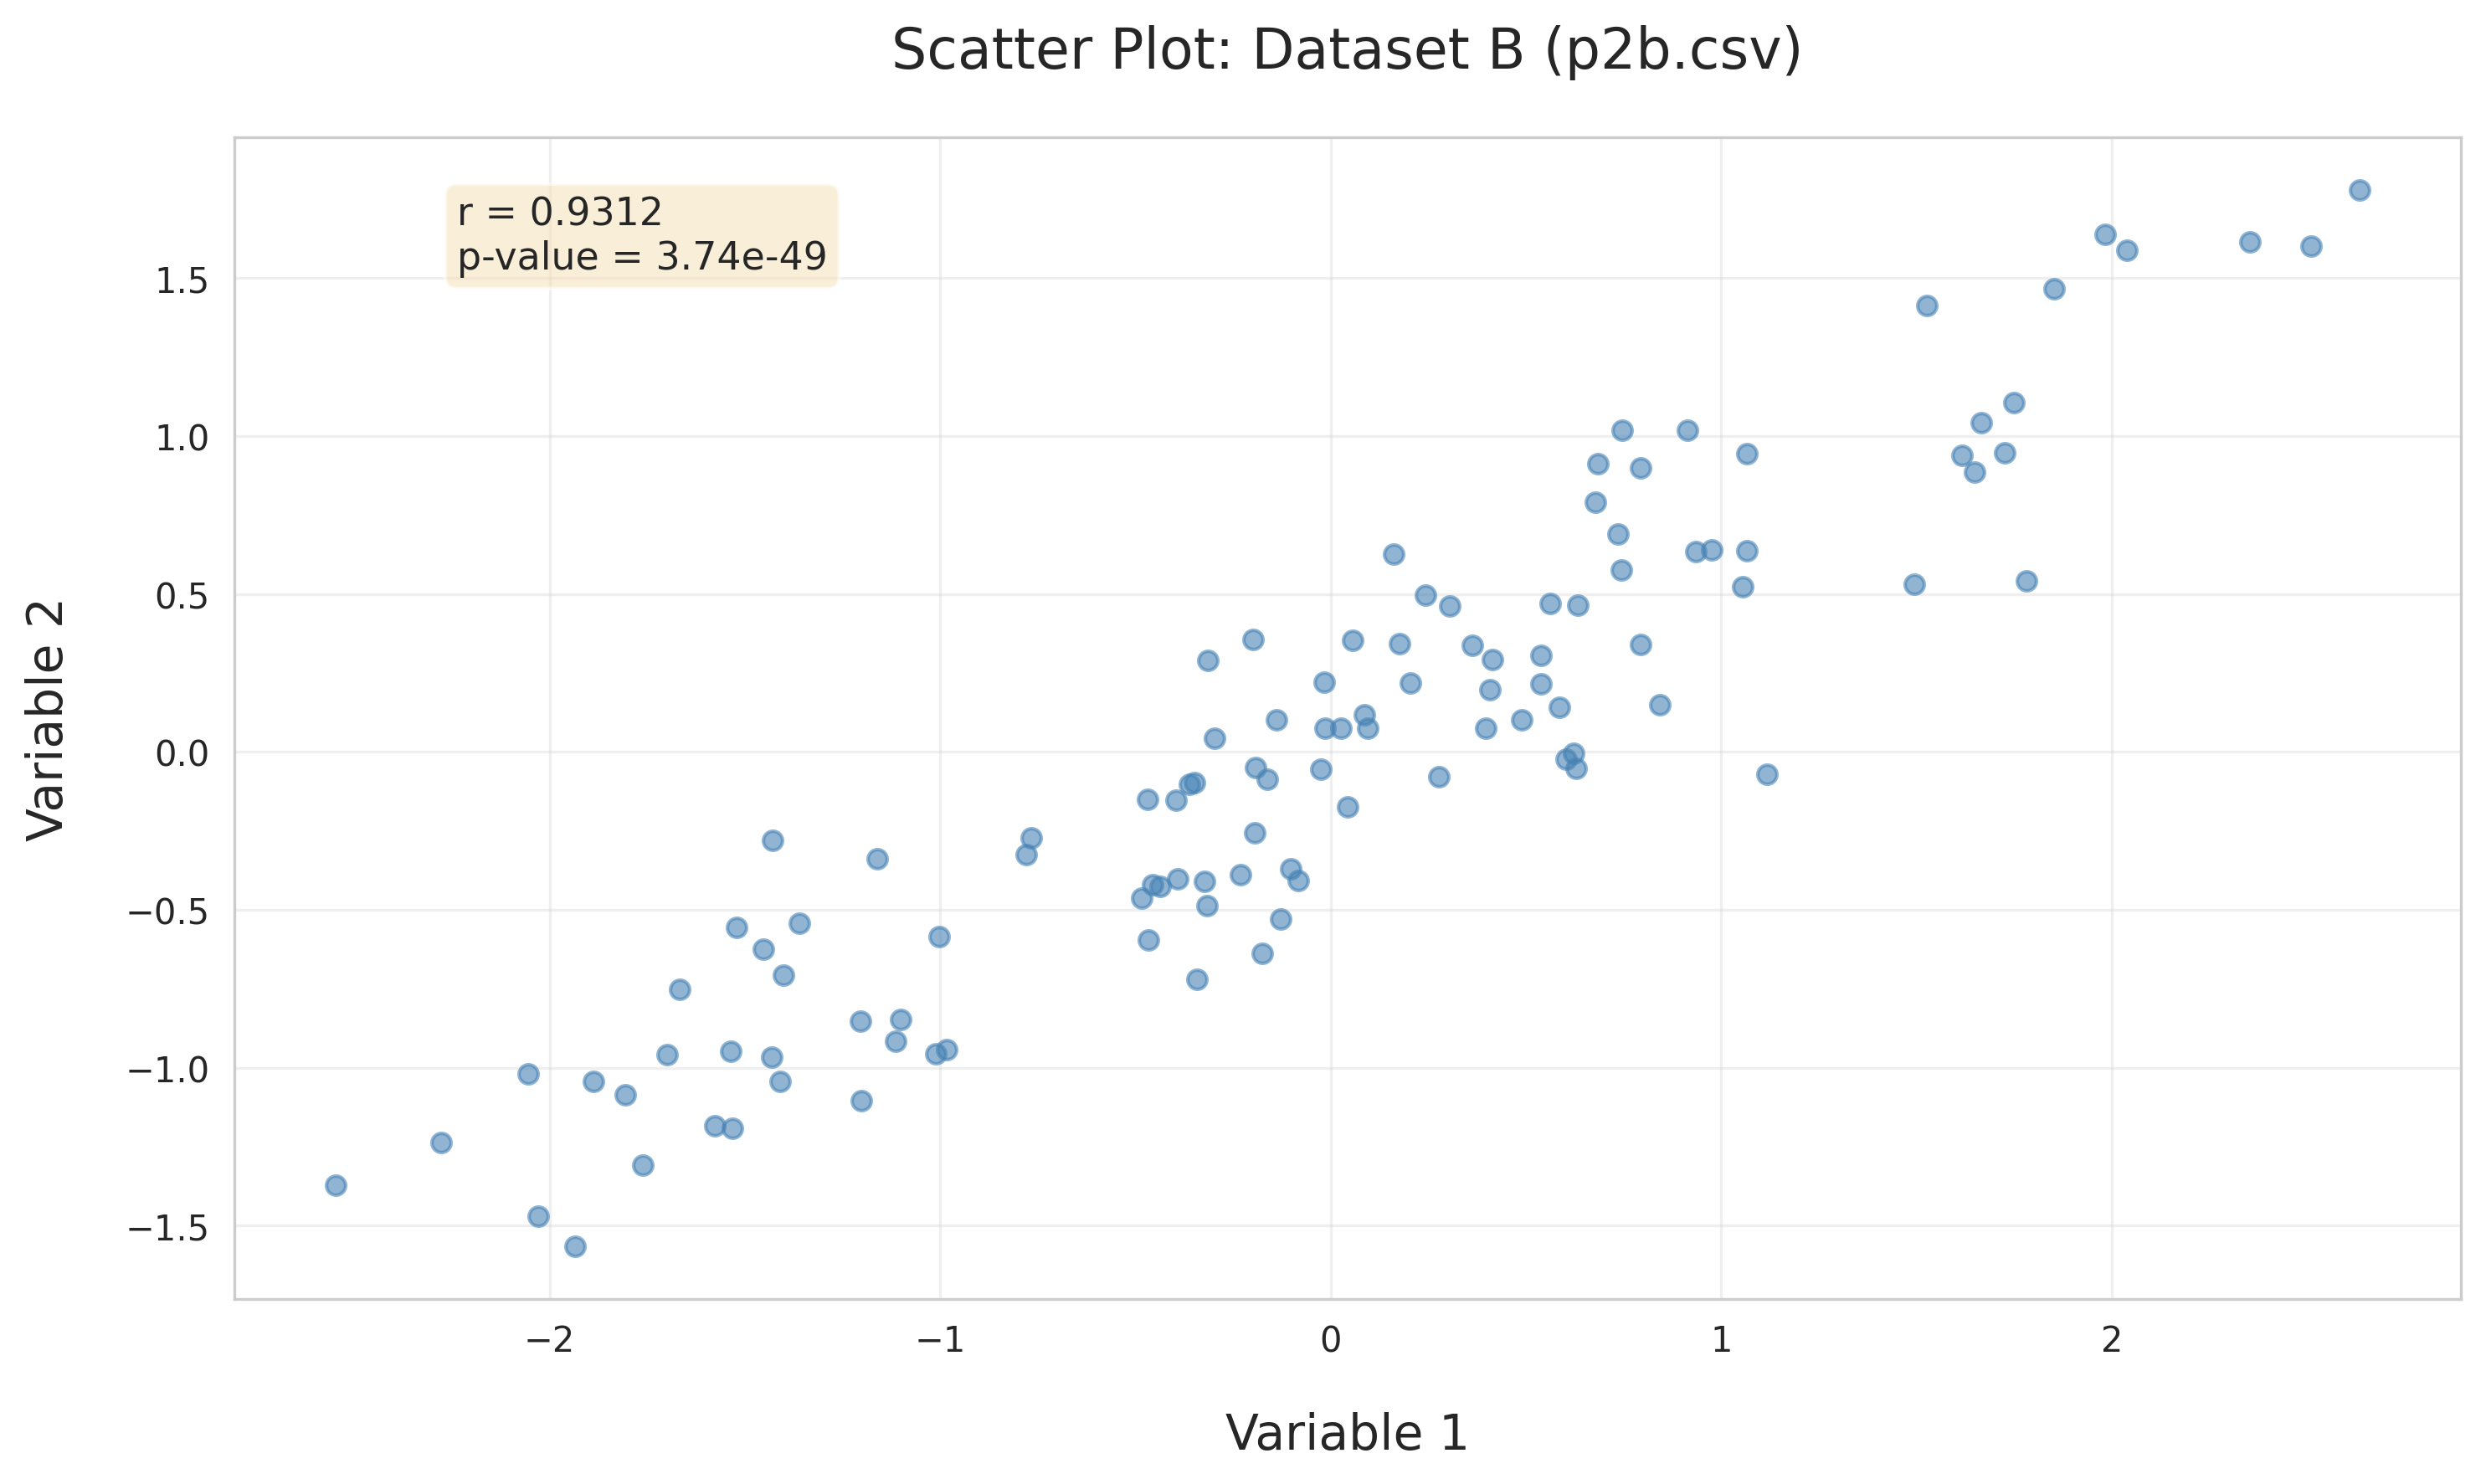
\includegraphics[width=0.95\textwidth]{figures/scatter_p2b.png}
    
    \textbf{Figure 5:} Scatter plot for p2b.csv.
\end{center}

The Pearson correlation for p2b came to 0.9312, and given the same significance level $ \alpha = 0.05 $, there is a statistically significant, positive association between the two variables. The p value $ p_b =  3.74 \times 10^{-49} $ is again much lower than the threshold, so we can confidently reject the null hypothesis.\\

According to the raw correlations $ r_a = 0.3809 $ and $ r_b = 0.9312 $, the part b variable pair shows a stronger correlation. However, the p-values $ p_a =  1.04 \times 10^{-83} $ and $ p_b =  3.74 \times 10^{-49} $ suggest that the part a variable pair is much smaller and therefore shows a stronger association, so these criteria don't agree. The reason for this is the difference in statistical power that lies in the sample size. p2a contains 2400 samples, while p2b only has 110: so in the case of p2a, even a moderate correlation becomes much more statistically significant because there is much more evidence that the pattern in not occurring by chance, whereas p2b has much less data to rule out randomness at play contributing to the association, and so even such an extreme correlation cannot produce a lower p-value.\\

Regarding the scatter plots, I would say off visual inspection that p2b shows a much clearer relationship, albeit the graph is much more sparse. The data stick very closely to the trend line as you would expect for such a high correlation, whereas p2a shows some agreement generally in the positive direction but as a whole kind of bulges out and looks befitting of a sample that would yield a moderate correlation value. So, my visual assessment agrees with the correlation assessment and not the p-value assessment. The p-value in p2a is simply a product of a larger sample and ought not to be misconstrued as an indication of a stronger relationship. Not to mention that the strength of p-values does not lie in making claims about qualities of the data itself, but more so in the uncertainty we possess in such claims. For that reason, I think my visual assessment of the scatter plots makes sense.

\newpage
